One of the key components of this experiment is the fact that charged reaction products stay within the ion trap, allowing us to accumulate all stages of a reaction network. Direct identification of the species via fluorescence is ideal, as the signal is unambiguous, and generally unique to a species. Leaning on direct fluorescence becomes increasingly difficult as more and more species are introduced. In our particular case, it becomes prohibitively difficult, as we may expect to trap 10's of species at once, where in some cases, the exact reaction products are not known. To identify what is in our trap, we use a species agnostic detection method in the form of a time of flight mass spectrometer (TOF-MS). Our TOF apparatus design and electronics were extensively developed by Steven Schowalter and Christian Schneider of the Hudson group.\cite{Schowalter2012,Schneider2014}

The TOF works by switching the rod voltages from a trapping RF potential to one where the ions are ejected out of one side. When trapping, RF voltages are applied onto diagonal rods, while DC voltages on the others. During ejection, the trapping region turns into the acceleration region as adjacent pairs of rods ramp to constant voltages where the pair of "back" rods are at a higher potential than the pair of "front" rods seen in Figure \ref{fig: rod traces}. TOF's operating with higher $m/z \approx>100 $ need to have well matched HVDC values for the rods, without much concern over the rising voltages. In our experiment, due to the low $m/z$ of \ce{Be+}, the ions were extremely susceptible to mismatches in the rod voltages during the ramp up, requiring particularly good overlap seen in $\sim 0.8 - 1.2$ $\mu$s of Figure \ref{fig: rod traces}

\begin{figure}
	\centering
	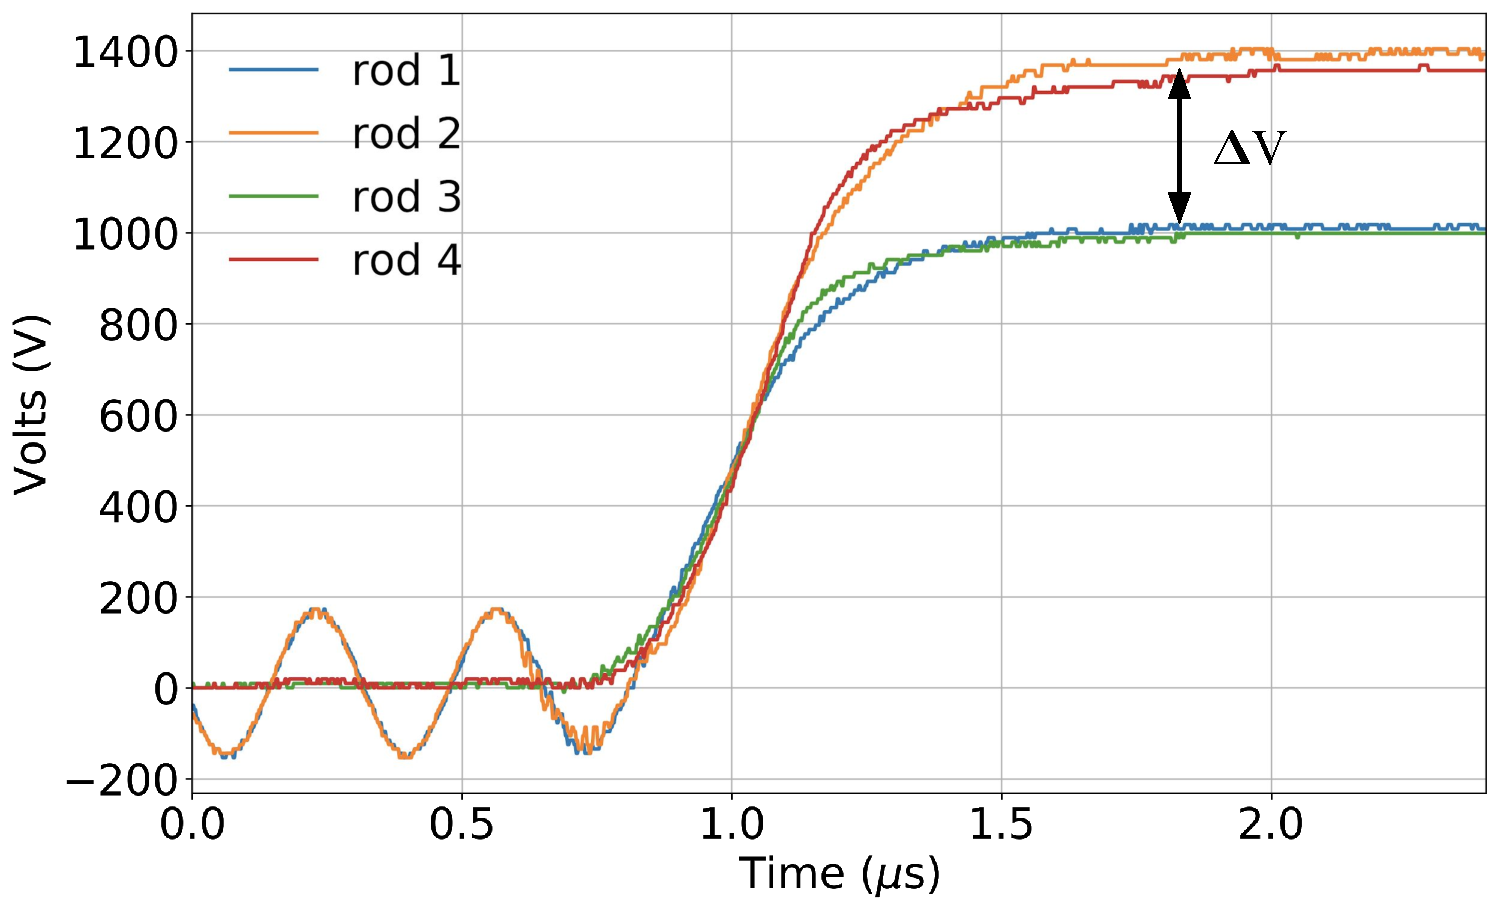
\includegraphics[width=0.8\textwidth]{images/rod_traces.pdf}
	\caption{Voltages of ion trap rods during ejection into the TOF taken from an oscilloscope. TOF facing front (1 and 3) and back (2 and 4) trap rod pairs shift from the trapping RF operation to HV values after a positive zero voltage crossing. The front pair reaches a nominal 1000 V, while the back pair reaches 1400 V, creating an accelerating potential $\Delta V$, ejecting the trapped ions.}
	\label{fig: rod traces}
\end{figure}

\begin{figure}
	\centering
	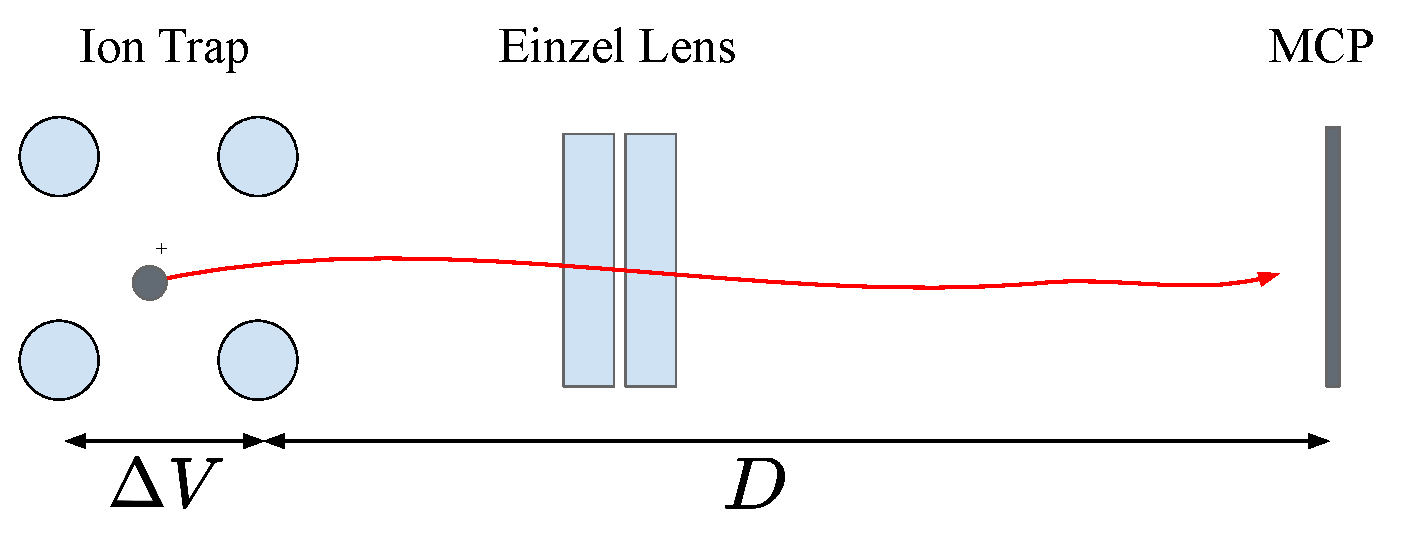
\includegraphics[width=0.8\textwidth]{images/TOF_diagram.pdf}
	\caption{Diagram of the TOF ejection where the ions in the trap are radially accelerated out of the trap with potential $\Delta V$. An Einzel lens ion focusing element focuses the ions onto the MCP at the back of the field free region of length $D$.}
	\label{fig: TOF diagram}
\end{figure}

As the ions are ejected radially, they are accelerated out of the trap, through an Einzel lens focusing element, and through a field-free drift tube of length $D=320$ mm where they impact a micro-channel plat (MCP) and are detected (Figure \ref{fig: TOF diagram}). To first order, during ejection the ions in the ion trap feel the same potential $\Delta V$, therefore, the same kinetic energy
\begin{equation*}
	\Delta V q = \frac{1}{2} m v^2.
\end{equation*}
But solving for the velocity $v$ yields a mass dependent velocity, thus, a mass dependent arrival time $t$,
\begin{align*}
	v & = \sqrt{\dfrac{2 \Delta V q}{m}} \\
	\implies t & = D \sqrt{\dfrac{m}{2 \Delta V q}}.
\end{align*}
With fast electronics, we may resolve ions to sub amu precision, giving us a powerful tool to identify what is in our trap. An example of \ce{Be+} and \ce{C+} TOF detection traces is shown in Figure \ref{fig: Be C TOF} with a ratio $m/\Delta m \approx 100$.

To first order, the mass to charge ratio ($m/z$) is then proportional to $t^2$ where $t$ is the arrival time, which is proportional to the drift tube length $D$. It may seem like greater mass separation is achieved with a longer drift tube, but that is not the case. We made the assumption that the ions are accelerated by the same potential, but in reality, the ions occupy a finite spacial extent in which the potential felt by an ion is related to its location within the trapping region at the time of ejection. An ion in the center of the trap at the time of ejection will have a distance $d_0\approx 4.8$ mm to travel in the acceleration region, while those towards the back/front pair of rods will have distances $d=d_0\pm \delta d$. As these ions fly down the drift tube, although the ions initially closer to the front have a shorter distance to travel, the ones originating further back have a higher velocity and will catch up and over take the slower ions. This mismatch will cause the ion arrival times of a single species to spread out as $D$ increases past the point where all the ions overlap.

On top of considering the spacial extent of the ions in the trap, we must also consider the multiple acceleration regions. The rods that the trap consists of produce a fairly uniform electric field within the trap region $E_d$, but outside, there is still an accelerating electric field $E_s$, but primarily from the front rods. To minimize the ion defocusing at the MCP, we find that the drift tube length $D$ is uniquely defined by the trap geometry and voltages,\cite{Wiley1955}
\begin{equation}
	D = 2d_0 k_0^{3/2}\left(1-\frac{1}{k+\sqrt{k}}\right)
\end{equation}
where $k = (E_s + E_d)/E_s$.

\subsection{TOF Signal Integration}

The MCP detector produces a current proportional to the number of ions that activate its surface, which is then read by a fast oscilloscope. To determine the total number of ions, we integrate the current as a function of arrival time to find a total charge for each calibrated amu range (colored regions in Figure \ref{fig: Be C TOF}). A difficulty is determining whether or not an integrated peak corresponds to an ion, or simply noise. For each TOF trace, we find a region of high mass (e.g. $m/z > 45$), where there aren't any ions and bin single amu chunks to produce a histogram. This histogram is then fitted to a Gaussian to determine the standard deviation, where then we may find a 90\% confidence interval ($\approx 1.3 \sigma$). This value then defines our signal threshold, if an integrated signal is below this value, it is rejected and a zero is returned with error bars equal to this threshold, otherwise it is reported as a true ion signal.